\section{Correlation}\label{sec:results}
Using Ca II H\&K emission data from \citet{Boudreaux2022} and
\citet{Perdelwitz2021} (quantified using the $R_{HK}$ metric) we investigate
the correlation between the Jao Gap magnitude and stellar magnetic activity. We
are more statistically limited here than past authors have been due to
the requirement for high resolution spectroscopic data when measuring Calcium
emission; however, this is balanced by the apparent stronger correlation between
Calcium emission and the Jao gap when compared to H$\alpha$ emission. 

The merged dataset is presented in Figure \ref{fig:mergedData}. There is a
visual discontinuity just below the Jao Gap magnitude; however, this
manifests as an increase in the spread of the emission measurements rather than
a change in the mean value. In order to quantify the significance of this
discontinuity we measure the false alarm probability of the change in standard
deviation.

\begin{figure}
  \centering
  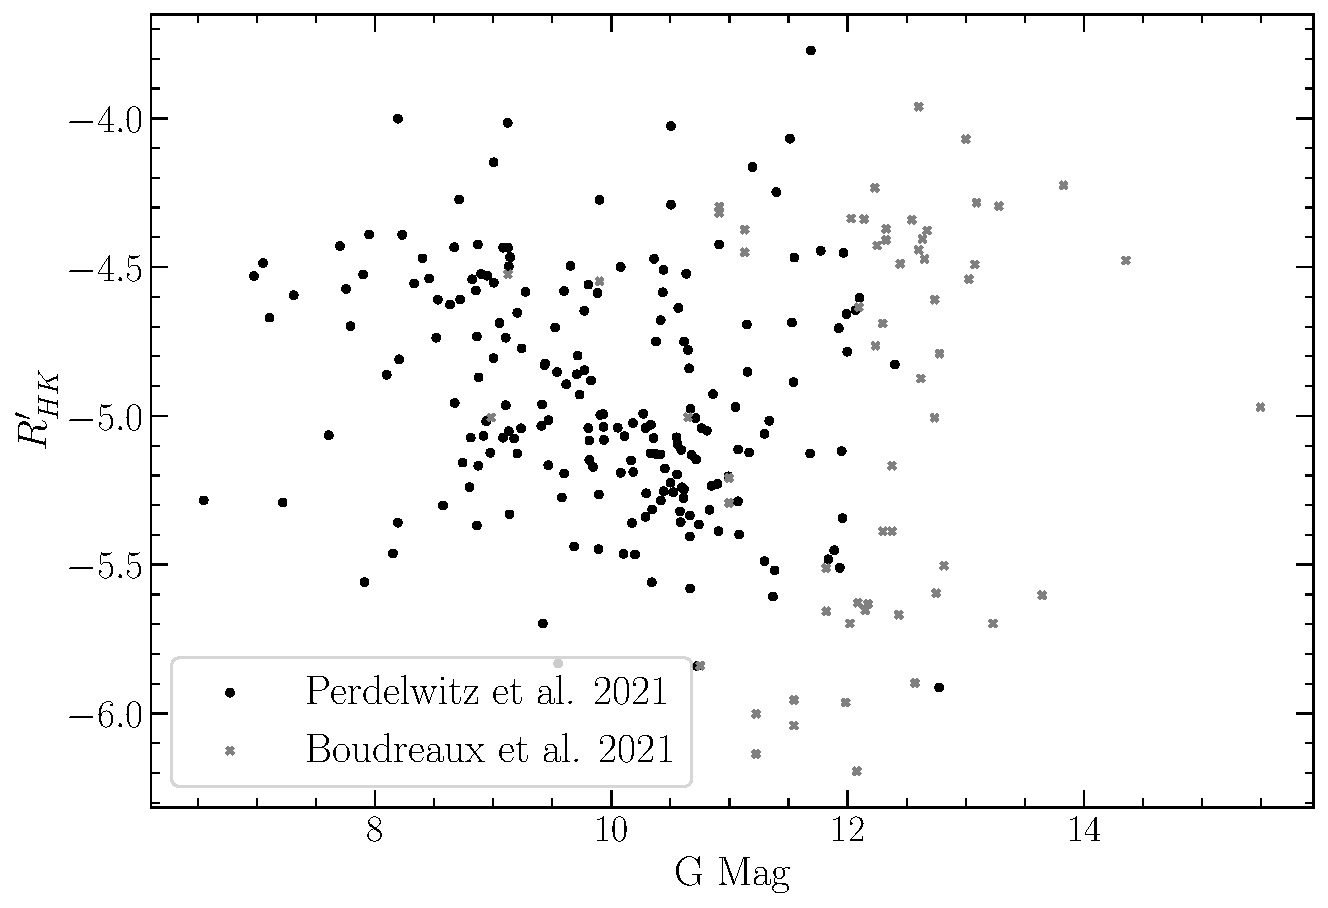
\includegraphics[width=0.45\textwidth]{figures/jaoMagActivity/Combined.pdf}
  \caption{Merged Dataset from \citet{Boudreaux2022, Perdelwitz2021}. Note the
  increase in the spread of $R'_{HK}$ around the Jao Gap Magnitude.}
  \label{fig:mergedData}
\end{figure}

First we split the merged dataset into bins with a width of 0.5 mag. In each bin we
measure the standard deviation about the mean of the data. The results of this
are shown in Figure \ref{fig:deviation}. In order to measure the false alarm
probability of this discontinuity we first resample the merged calcium
emission data based on the associated uncertainties for each datum as
presented in their respective publications. Then, for each of these ``resample
trials'' we measure the probability that a change in the standard deviation of
the size seen would happen purely due to noise. Results of this test are show in
in Figure \ref{fig:dist}. 

\begin{figure}
  \centering
  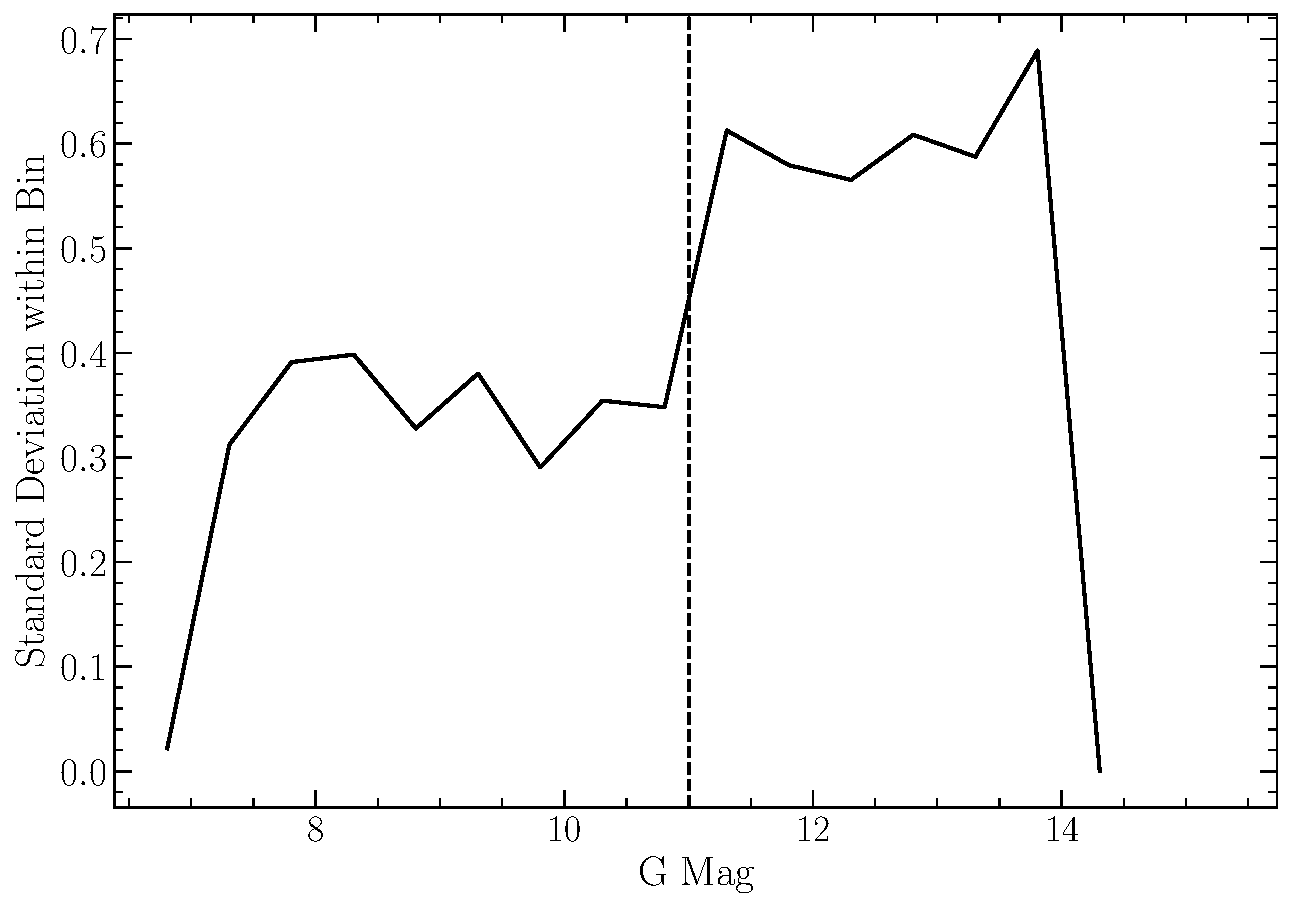
\includegraphics[width=0.45\textwidth]{figures/jaoMagActivity/Deviation.pdf}
  \caption{Standard deviation of Calcium emission data within each bin. Note
  the discontinuity near the Jao Gap Magnitude.}
  \label{fig:deviation}
\end{figure}

\begin{figure}
  \centering
  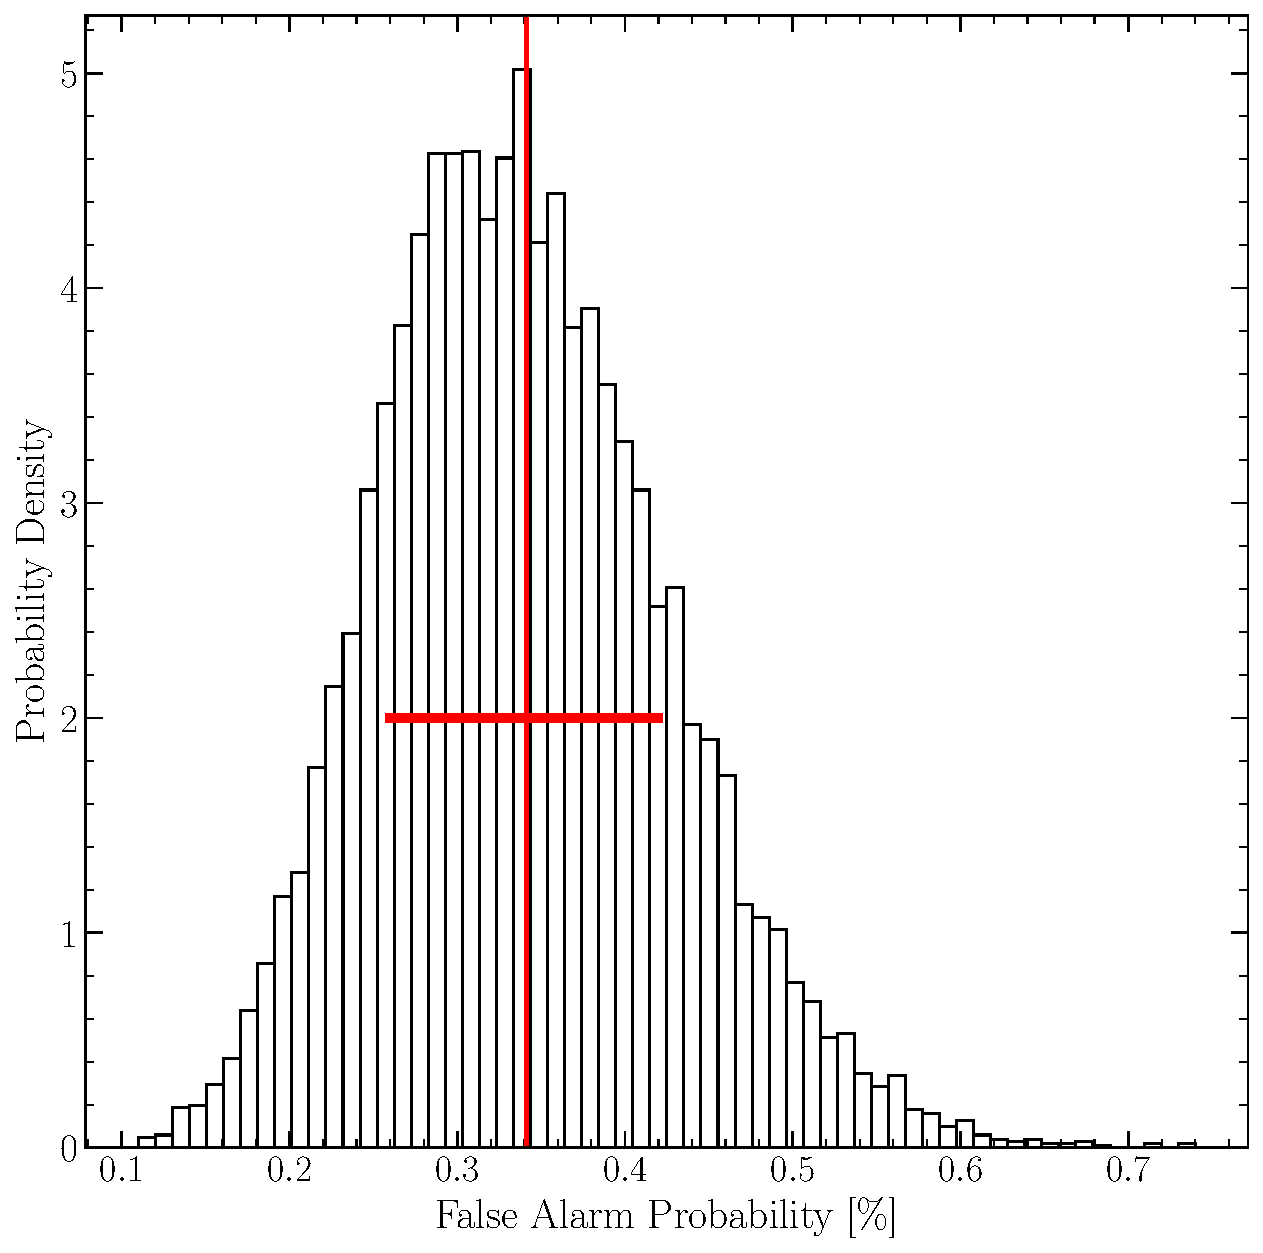
\includegraphics[width=0.45\textwidth]{figures/jaoMagActivity/fpDist.pdf}
  \caption{Probability distribution of the false alarm probability for the
  discontinuity seen in Figure \ref{fig:deviation}. The mean of this
  distribution is $0.341\%\pm^{0.08}_{0.08}$.}
  \label{fig:dist}
\end{figure}

This rapid increase star-to-star variability would only arise due purely to
noise $0.3\pm0.08$ percent of the time and is therefore likely either a true
effect or an alias of some sample bias. {\color{red} COME BACK TO HERE TO FLUSH
OUT SAMPLE BIAS SECTION.}

If the observed increase in variability is not due to a sample bias and rather
is a physically driven effect then there is an obvious similarity between these
findings and those of \citep{Jao2023}. Specifically we find a increase in
variability just below the magnitude of the gap. Moreover, this variability
increase is primarily driven by an increase in the number of low activity stars
(as opposed to an increase in the number of high activity stars). We can
further investigate the observed change in variability for only low activity
stars by filtering out those stars at or above the saturated threshold for
magnetic activity. \citet{Boudreaux2022} identify $\log(R'_{HK}) = -4.436$ as
the saturation threshold. We adopt this value and filter out all stars where
$\log(R'_{HK}) \geq -4.436$. Applying the same analysis to this reduced dataset
as was done to the full dataset we still find a discontinuity at the same
location (Figure \ref{fig:reduced}). This discontinuity is of a smaller
magnitude and consequently is more likely to be due purely to noise, with a
$7\pm0.2$ percent false alarm probability. This false alarm probability is
however only concerned with the first point after the jump in variability. If
we consider the false alarm probability of the entire high variability region
then the probability that the high variability region is due purely to noise
drops to $1.4\pm0.04$ percent.

\begin{figure}
  \centering
  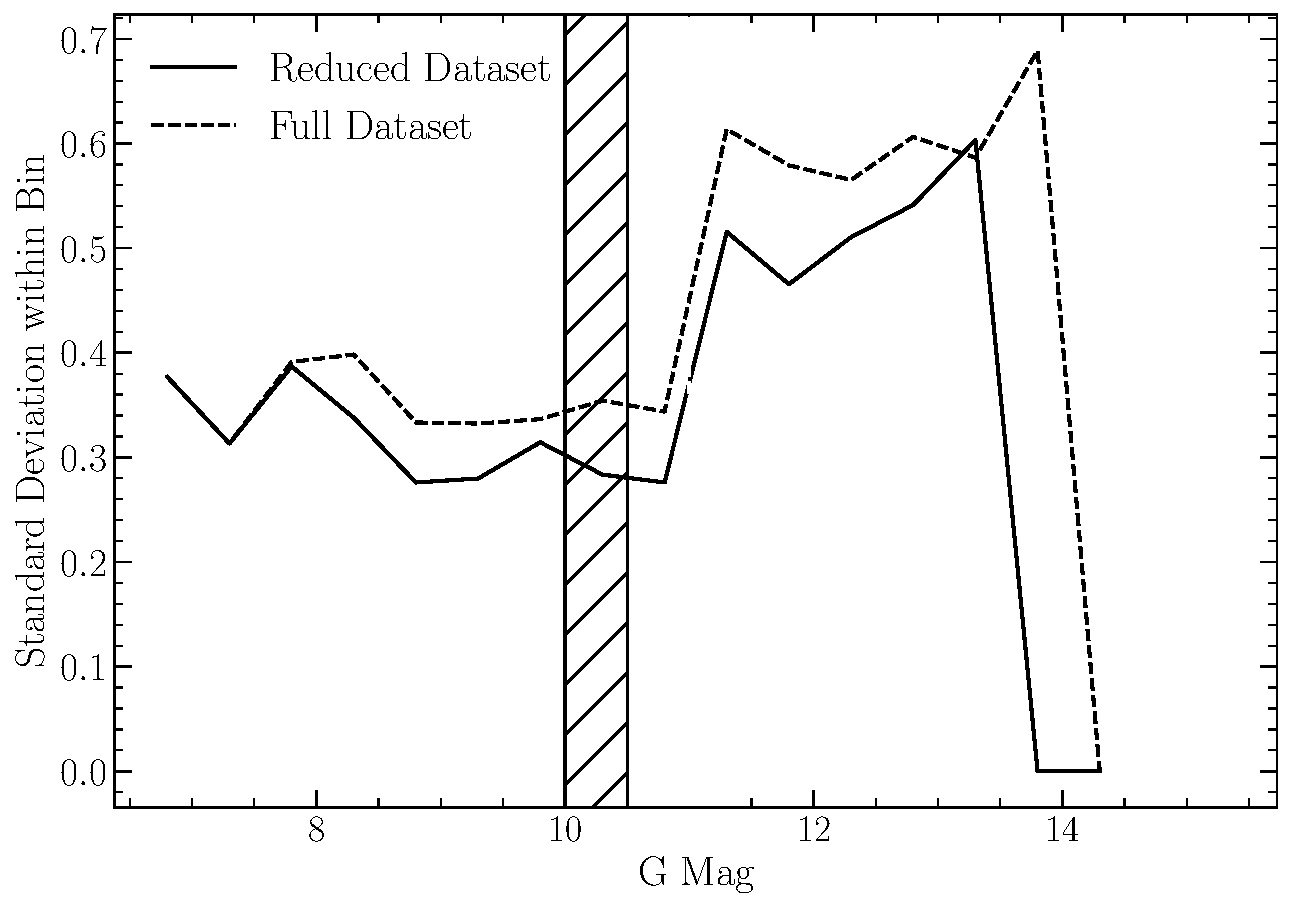
\includegraphics[width=0.45\textwidth]{figures/jaoMagActivity/ReducedDeviation.pdf}
  \caption{Spread in the magnetic activity metric for the merged sample with
  any stars $\log(R'_{HK}) > -4.436$ filtered out.}
  \label{fig:reduced}
\end{figure}

We observe a strong, likely statistically significant, discontinuity in the
star-to-star variability of Ca II K \& K emission just below the magnitude
of the Jao Gap. However, modeling is required to determine if this discontinuity
may be due to the same underlying physics.

While the observed increase in variability seen here does not seem to be
coincident with the Jao Gap --- instead appearing to be approximately 0.5 mag
fainter, in agreement with what is observed in \citet{Jao2023} --- a number of
complicating factors prevent us from falsifying that the these two features are
not coincident. \citeauthor{Jao2023} find, similar to the results presented
here, that the paucity of $H\alpha$ emission originates just below the gap.
Moreover, we use a 0.5 magnitude bin size when measuring the star-to-star
variability which injects error into the positioning of any feature in
magnitude space. We can quantify the degree of uncertainty the magnitude bin
choice injects by conducting Monte Carlo trials where bins are randomly shifted
redder or bluer. We conduct 10,000 trials where each trial involves sampling a
random shift to the bin start location from a normal distribution with a
standard deviation of 1 magnitude. For each trial we identify the discontinuity
location as the maximum value of the gradient of the standard deviation
(effectively this is just the derivative of \ref{fig:reduced}). Some trials
result in the maximal value lying at the 0th index of the magnitude array due
to edge effects, these trials are rejected (and account for 11\% of the
trials). The uncertainty in the identified magnitude of the discontinuity due
to the selected start point of the magnitude bins reveals a $1\sigma = \pm$0.32
magnitude uncertainty in the location of the discontinuity (Figure
\ref{fig:GapLocationMC}). Finally, all previous studies of the M dwarf gap
\citep{Jao2018, Feiden2022, Mansfield2021, Boudreaux2022, Jao2023} demonstrate
that the gap has a color dependency, shifting to fainter magnitudes as the
population reddens and consequently an exact magnitude range is ill-defined.
Therefore we cannot falsify the model that the discontinuity in star-to-star activity
variability is coincident with the Jao Gap magnitude.

\begin{figure}
  \centering
  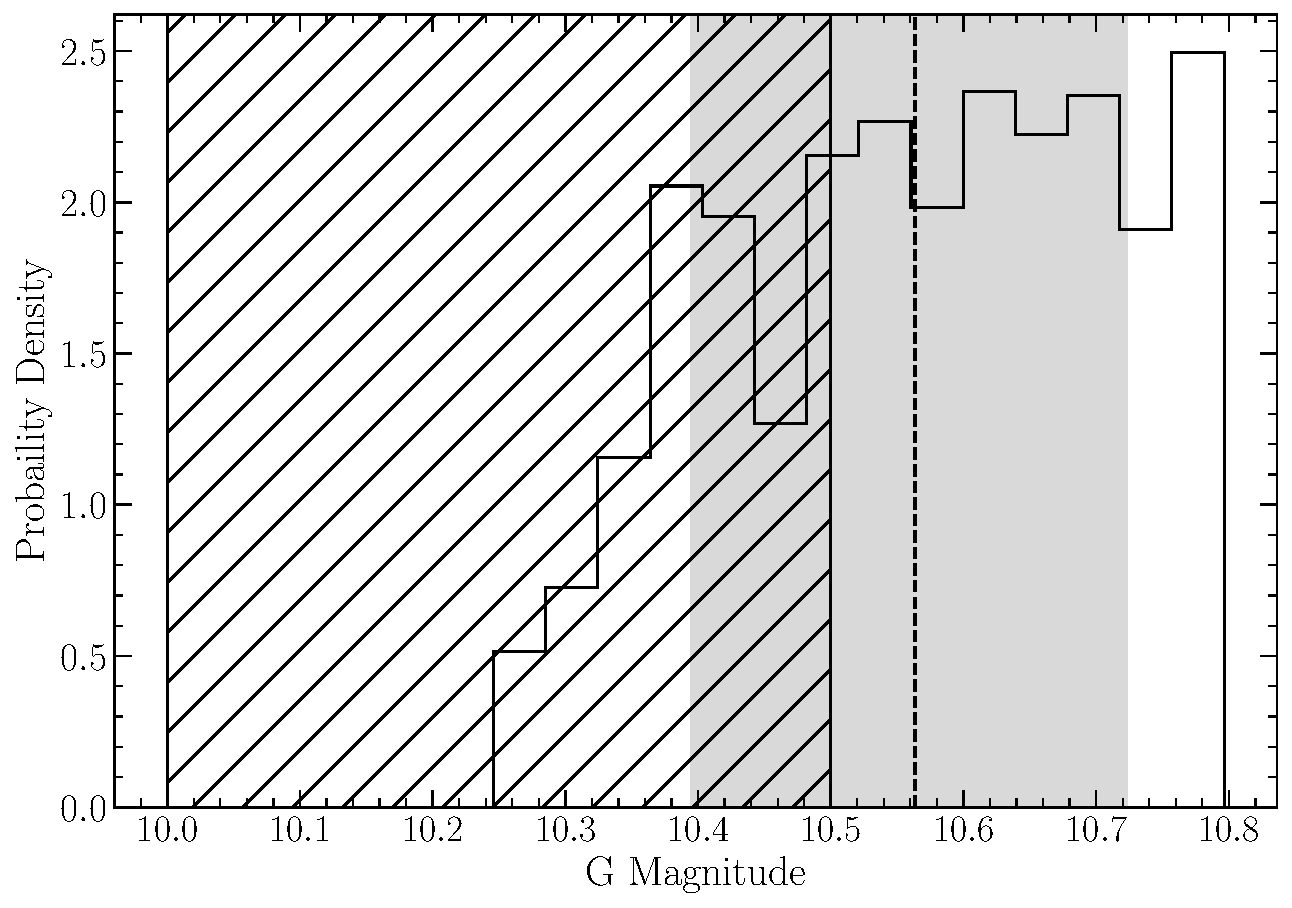
\includegraphics[width=0.45\textwidth]{figures/jaoMagActivity/GapLocationMC.pdf}
  \caption{Probability density distribution of discontinuity location as
  identified in the merged dataset. The dashed line represents the mean of the
  distribution while the shaded region runs from the 16th percentile to the
  84th percentile of the distribution. This distribution was built from 10,000
  independent samples where the discontinuity was identified as the highest
  value in the gradient of the standard deviation.}
  \label{fig:GapLocationMC}
\end{figure}

\subsection{Rotation}
Following the process described in \citet{023AJ....165..192G}, we first put the
dataset through \texttt{stella} \citep{FeinsteinFlare2020,FeinsteinStella2020},
a convolutional neural network that trains a multitude of models, given a
different initial seed, on TESS 2-min cadence. In this case, we also used an
ensemble of 100 models to optimize the gains. \texttt{stella} identifies flares
given a score of 0 to 1, here we use a score of 0.5 and above as flare
identification. Furthermore, we also bin the data from a 2-min to 10-min
cadence using \texttt{lightkurve}'s binning function
\citep{LightkurveCollaborationLightkurve2018,GeertBarentsenKeplerGO2020}. Not
only does this help further reduce any flaring-contribution that might have
been missed by \texttt{stella}\footnote{This is relevant for flares that are
misshapen at the start or break in the dataset due to missing either the
ingress or egress.}, but it also optimizes computational efficiency.
Subsequently, we calculate residuals by subtracting the model from the data,
retaining data with residuals smaller than 4 times the root-mean-square.

As M dwarfs often exhibit non-sinusoidal and quasi-periodic rotational
variability, we employ Gaussian processes for modeling based on
\citet{AngusInferring2018} for the subset of M Dwarfs with no fiducial periods.
The \texttt{starspot} \ package is adapted for light curve analysis
\citep{AngusRuthAngus2021,https://doi.org/10.5281/zenodo.7697238} and
accessible at (HAVEN'T DONE IT YET-AYLIN). Our Gaussian process kernel function
incorporates two stochastically-driven simple harmonic oscillators,
representing primary ($P_\textrm{rot}$) and secondary ($P_\textrm{rot}/2$)
rotation modes. First, we implement the Lomb-Scargle periodogram within
\texttt{starpot} to initially estimate the period. After which, we create a
maximum a posteriori (MAP) fit using \texttt{starspot} to generate a model for
stellar rotation. To obtain the posterior of the stellar rotation model, we use
Markov Chain Monte Carlo (MCMC) sampling using the \texttt{pymc3} package
\citep{SalvatierProbabilistic2016} within our adapted \texttt{starspot}
version. 

ANALYSIS PART YET TO BE DETERMINED.

\subsection{Limitations}
There are two primary limitation of our dataset. First, we only have
{\color{red}232 stars} in our dataset limiting the statistical power of our
analysis. This is primarily due to the relative difficulty of obtaining Ca II
H\&K measurements compared to obtaining $H\alpha$ measurements. Reliable
measurements require both high spectral resolutions ({\color{red} R $\sim$
XXXXXX}) and a comparatively blue wavelength range \footnote{wrt. too what many
spectrographs cover. There is no unified resource listing currently
commissioned spectrographs; however, it is somewhat hard to source glass which
transmits well at H\&K wavelengths limiting the lower wavelength of most
spectrographs.}.

Additionally, the sample we do have does not extend to as low mass as would be
ideal. This presents a degeneracy between two potential causes for the observed
increased star-to-star variability. One option, as presented above and
elaborated on in the following section, is that this is due to kissing
instabilities. However, another possibility is that this increased variability
is intrinsic to the magnetic fields of fully convective stars. There is limited
discussion in the literature of the latter effect; however, \citet{Shulyak2019}
present estimated magnetic field strengths for 47 M dwarfs, spanning a larger
area around the convective transition region and their dataset does not
indicate a inherently increased variability for fully convective stars
({\color{red} fully confirm this, not just visually}).
